\chapter{Trường lượng tử cục bộ và phương trình Dirac một chiều}

Ta đã làm quen với trường lượng tử thông qua các lượng tử của chúng, các toán tử sinh và hủy, cùng Hamiltonian đơn giản nhất cho các hạt phi tương đối tính. Giờ đây, ta sẽ vận dụng bộ công cụ ấy. Trước hết, thay vì chỉ khẳng định, ta sẽ thấy Hamiltonian cục bộ theo không gian bảo toàn động lượng như thế nào. Sau đó, ta sẽ dùng tích các trường để mô tả tán xạ và phân rã, đồng thời theo dõi cách tác dụng lặp lại của Hamiltonian tạo nên những bước đầu của lý thuyết nhiễu loạn bằng giản đồ. Chỉ sau đó ta mới chuyển sang bài toán fermion đã hứa. Lối vào rõ ràng nhất chưa phải là trường fermion, mà là phương trình Dirac một chiều.

\section{Nhắc lại Hamiltonian trường}

Viết Hamiltonian cho một loài hạt phi tương đối tính như sau:
\begin{equation}
H_0=\int dx\,
\psi^\dagger(x)
\left[-\frac{\partial_x^2}{2m}+V(x)\right]
\psi(x).
\label{eq:l9-nonrel-hamiltonian}
\end{equation}
Ký hiệu trông như chỉ áp dụng trong một chiều, nhưng không gì trong lập luận mở đầu phụ thuộc vào hạn chế đó: trong ba chiều, \(x\) có thể chỉ vectơ \(\mathbf{x}\), \(dx\) chỉ \(d^3x\), còn \(-\partial_x^2\) chỉ \(-\nabla^2\).

Toán tử \(\psi^\dagger(x)\) tạo một hạt tại \(x\), còn \(\psi(x)\) hủy một hạt tại đó. Tích được sắp thứ tự chuẩn tắc của chúng,
\begin{equation}
n(x)=\psi^\dagger(x)\psi(x)
\end{equation}
là mật độ số cục bộ. Vì thế, số hạng thế năng có dạng
\begin{equation}
H_V=\int dx\,V(x)n(x).
\end{equation}
Đây chính xác là cách viết cho một khí cổ điển: đếm các hạt gần \(x\), gán cho mỗi hạt thế năng \(V(x)\), rồi cộng trên toàn không gian. Ở giai đoạn này, các hạt không tương tác với nhau. Chúng có thể chịu tác động của một thế năng áp đặt từ bên ngoài, nhưng ngoài ra Hamiltonian chỉ là tổng các năng lượng một hạt độc lập.

Ta có thể giản lược bài toán rồi quay lại điểm xuất phát. Chọn thế năng là hằng số, \(V(x)=V_0\). Thế năng hằng không gây lực, nhưng ý nghĩa toán tử của nó rất rõ ràng:
\begin{equation}
\begin{aligned}
H_V&=V_0\int dx\,\psi^\dagger(x)\psi(x)=V_0N,\\
N&=\int dx\,n(x).
\end{aligned}
\end{equation}
Nó cộng thêm cùng một năng lượng cho mỗi hạt. Để giữ năng lượng nghỉ trong mô tả phi tương đối tính, chọn \(V_0=mc^2\). Khi đó, số hạng này tính một năng lượng nghỉ cho mỗi hạt. Ta giữ lại hằng số vốn khá tẻ nhạt này vì nó bảo toàn tính bất biến tịnh tiến và làm cho phép đếm số hạt hiện rõ.

\section{Hamiltonian như một quy tắc cập nhật}

Bảo toàn động lượng có nghĩa là gì? Ta nên diễn đạt câu trả lời qua tác dụng của Hamiltonian. Để tránh dùng \(\psi\) cùng lúc cho toán tử trường, hàm sóng một hạt và trạng thái nhiều hạt, ta ký hiệu trạng thái nhiều hạt là \(\lvert\Phi(t)\rangle\). Trong một khoảng thời gian ngắn \(\epsilon\),
\begin{equation}
\lvert\Phi(t+\epsilon)\rangle
=\left(1-i\epsilon H+O(\epsilon^2)\right)
\lvert\Phi(t)\rangle,
\label{eq:l9-short-update}
\end{equation}
trong đó \(\hbar=1\). Số hạng thứ nhất là trạng thái không đổi; hiệu chỉnh đầu tiên do \(H\) sinh ra. Lặp đi lặp lại phép cập nhật này sẽ cho phương trình Schr\"odinger.

Giờ đây, bảo toàn động lượng có ý nghĩa cụ thể. Nếu trạng thái ban đầu có tổng động lượng xác định \(P\), thì \(H\lvert\Phi\rangle\) cũng phải có cùng tổng động lượng ấy. Các tính chất khác có thể thay đổi, và từng hạt có thể trao đổi động lượng, nhưng Hamiltonian không thể đưa trạng thái sang một phân khu có tổng \(P\) khác. Ta có thể kiểm tra trực tiếp điều này bằng cách viết lại Hamiltonian trong cơ sở động lượng.

\section{Tích phân không gian thành hàm delta động lượng}

Chọn quy ước Fourier
\begin{align}
\psi(x)&=\int\frac{dp}{\sqrt{2\pi}}\,a(p)e^{ipx},\\
\psi^\dagger(x)&=\int\frac{dq}{\sqrt{2\pi}}\,a^\dagger(q)e^{-iqx}.
\label{eq:l9-field-fourier}
\end{align}
Toán tử \(a(p)\) hủy một hạt có động lượng \(p\).
Toán tử \(a^\dagger(q)\) tạo một hạt có động lượng \(q\). Việc dùng các ký hiệu khác nhau là thiết yếu: hai động lượng được lấy tích phân độc lập cho đến khi tích phân không gian liên hệ chúng với nhau.

Bắt đầu với số hạng số hạt:
\begin{align}
N
&=\int dx\,\psi^\dagger(x)\psi(x)\\
&=\int\frac{dp\,dq}{2\pi}\,
a^\dagger(q)a(p)
\int dx\,e^{i(p-q)x}.
\end{align}
Tích phân còn lại là
\begin{equation}
\int dx\,e^{i(p-q)x}=2\pi\delta(p-q).
\end{equation}
Khi \(p\ne q\), pha dao động và các đóng góp dương, âm triệt tiêu nhau. Khi \(p=q\), pha hoàn toàn không dao động. Phân bố delta Dirac là đối tượng chính xác kết hợp hai sự thật đó. Do đó,
\begin{align}
N
&=\int dp\,dq\,a^\dagger(q)a(p)\delta(p-q)\\
&=\int dp\,a^\dagger(p)a(p).
\label{eq:l9-number-momentum}
\end{align}
Toán tử hủy một hạt có động lượng \(p\) rồi tạo lại một hạt đúng cùng động lượng ấy. Yếu tố quyết định là tích phân theo \(x\): nó tạo ra hàm delta buộc động lượng đi vào phải bằng động lượng đi ra.

\begin{classroomqa}\lecturetimestamp{00:17:02}\audiencequestion{Vô hạn xuất hiện khi \(p=q\) đã đi đâu?}\lecturerresponse{Không thể dùng hàm delta bằng cách lấy giá trị chiều cao của nó. Đây là một phân bố được định nghĩa thông qua phép tích phân: \(\int dk\,\delta(k)f(k)=f(0)\). Cụm từ ``cao vô hạn và hẹp vô hạn'' chỉ nhắc ta rằng trọng số tích phân của nó bằng một. Ở đây, nó yêu cầu ta đặt \(p-q=0\), và không còn kết quả vô hạn nào.}\end{classroomqa}

Cơ chế tương tự áp dụng cho một đơn thức cục bộ tổng quát hơn nhiều. Giả sử một số hạng chứa vài trường hủy và vài trường tạo, có thể thuộc những loài khác nhau, nhưng tất cả đều được tính tại cùng một điểm và tích phân theo điểm đó:
\begin{equation}
\int dx\,
\prod_{r=1}^{n} \psi_{i_r}^\dagger(x)
\prod_{s=1}^{m} \psi_{j_s}(x).
\end{equation}
Gọi động lượng của các hạt bị hủy là \(p_s\) và của các hạt được tạo là \(q_r\). Khai triển Fourier cho
\begin{equation}
\int dx\,
e^{i(\sum_s p_s-\sum_r q_r)x}
=2\pi\,
\delta\!\left(\sum_s p_s-\sum_r q_r\right).
\label{eq:l9-total-momentum-delta}
\end{equation}
Kết quả không ghép \(p_1\) với \(q_1\), \(p_2\) với \(q_2\), vân vân. Nó chỉ áp đặt điều kiện
\begin{equation}
\sum_{\mathrm{annihilated}}p
=
\sum_{\mathrm{created}}q.
\end{equation}
Đó chính là quy tắc cần có cho một tương tác: động lượng riêng lẻ có thể thay đổi, nhưng tổng động lượng thì không. Phát biểu sâu xa hơn là tính bất biến tịnh tiến. Một mật độ cục bộ được tích phân với cùng trọng số tại mọi điểm không có gốc tọa độ ưu tiên, và biến đổi Fourier của nó mang theo hàm delta bảo toàn động lượng tương ứng.

\begin{classroomqa}\lecturetimestamp{00:23:04}\audiencequestion{Số hạng Hamiltonian được đề xuất có thực sự là tích của tất cả các toán tử trường ấy không? Vì sao ta lại viết tích như vậy?}\lecturerresponse{Đúng vậy. Tích này chỉ rõ những hạt nào bị loại bỏ và những hạt nào được tạo ra tại cùng một điểm. Động cơ vật lý của nó sẽ đến từ các quá trình tán xạ hoặc phân rã quan sát được; ta xác lập lập luận về động lượng trước để có thể nhận ra ngay các tương tác ấy.}\end{classroomqa}

\section{Động năng trong không gian động lượng và không gian vị trí}

Giờ hãy áp dụng cùng bộ công cụ cho số hạng đạo hàm. Đạo hàm tác dụng lên sóng phẳng:
\begin{equation}
-\partial_x^2 e^{ipx}=p^2e^{ipx}.
\end{equation}
Do đó,
\begin{align}
H_{\mathrm{kin}}
&=\int dx\,\psi^\dagger(x)
\left(-\frac{\partial_x^2}{2m}\right)\psi(x)\\
&=\int dp\,\frac{p^2}{2m}\,a^\dagger(p)a(p).
\label{eq:l9-kinetic-momentum}
\end{align}
Một lần nữa, tích phân không gian buộc động lượng đi vào và đi ra bằng nhau. Thừa số mới \(p^2/2m\) chỉ đơn giản gán trọng số là động năng của mỗi mode cho số hạt trong mode đó.

\begin{classroomqa}\lecturetimestamp{00:24:46}\audiencequestion{Lấy đạo hàm sóng phẳng hai lần có phải cho dấu trừ không?}\lecturerresponse{Đúng, \(\partial_x^2e^{ipx}=-p^2e^{ipx}\). Hamiltonian vốn đã chứa dấu trừ bù lại, nên \(-\partial_x^2\) có trị riêng dương \(p^2\).}\end{classroomqa}

\begin{classroomqa}\lecturetimestamp{00:27:20}\audiencequestion{Động năng chỉ được bảo toàn khi thế năng là hằng số thôi sao?}\lecturerresponse{Đúng. Khi không có thế năng phụ thuộc vị trí, không có lực và động năng được bảo toàn riêng. Trong một thế năng ngoài không hằng, động năng và thế năng có thể trao đổi với nhau, trong khi Hamiltonian toàn phần vẫn được bảo toàn nếu nó không phụ thuộc tường minh vào thời gian.}\end{classroomqa}

\begin{classroomqa}\lecturetimestamp{00:27:42}\audiencequestion{\(\psi^\dagger\psi\) có vai trò gì trong Hamiltonian động năng biểu diễn theo động lượng?}\lecturerresponse{Đó là toán tử đếm. Tích mode \(a^\dagger(p)a(p)\) đếm số hạt có động lượng \(p\), còn thừa số \(p^2/2m\) gán động năng thích hợp cho mỗi hạt.}\end{classroomqa}

Có một cách thứ hai để thấy tính dương. Tích phân từng phần một lần và bỏ qua số hạng biên, ta được
\begin{align}
\int dx\,\psi^\dagger(-\partial_x^2)\psi
&=\int dx\,(\partial_x\psi^\dagger)(\partial_x\psi).
\label{eq:l9-positive-kinetic}
\end{align}
Với các trường triệt tiêu đủ nhanh ở vô cực, hoặc với điều kiện biên tuần hoàn, phần biên bằng không. Kết quả có dạng bình phương môđun và không âm. Nó cũng cho thấy một kiểu biểu thức thường gặp trong lý thuyết trường: năng lượng chứa bình phương các đạo hàm không gian của trường.

\section{Tương tác tiếp xúc cục bộ}

Giờ hãy giao cho các tích trường một nhiệm vụ vật lý. Xét hai loài hạt, ta tạm gọi là electron và proton để hình dung cho quen thuộc. Trước mắt, chúng được cố ý mô hình hóa không đúng thực tế: cả hai đều được mô tả bằng các toán tử boson, còn tương tác Coulomb thực sự bị bỏ qua. Hamiltonian tự do của chúng là
\begin{equation}
H_0=\int dx\left[
\psi_e^\dagger\left(-\frac{\partial_x^2}{2m_e}\right)\psi_e
+
\psi_p^\dagger\left(-\frac{\partial_x^2}{2m_p}\right)\psi_p
\right].
\end{equation}
Thêm tương tác mô hình
\begin{equation}
H_{\mathrm{contact}}
=g\int dx\,
\psi_e^\dagger(x)\psi_p^\dagger(x)
\psi_e(x)\psi_p(x).
\label{eq:l9-contact}
\end{equation}
Đọc biểu thức từ phải sang trái. Nó tìm một electron và một proton tại cùng điểm \(x\), hủy cả hai rồi tạo lại chúng tại điểm ấy. Nếu hai hạt không ở cùng nhau, số hạng cục bộ này cho kết quả bằng không. Nếu các đường thế giới của chúng gặp nhau, nó có thể làm thay đổi động lượng riêng lẻ của chúng mà vẫn bảo toàn tổng động lượng. Vì vậy, nó đóng vai trò như một thế tán xạ lý tưởng hóa có tầm tác dụng bằng không.

\begin{figure}[htbp]\centering
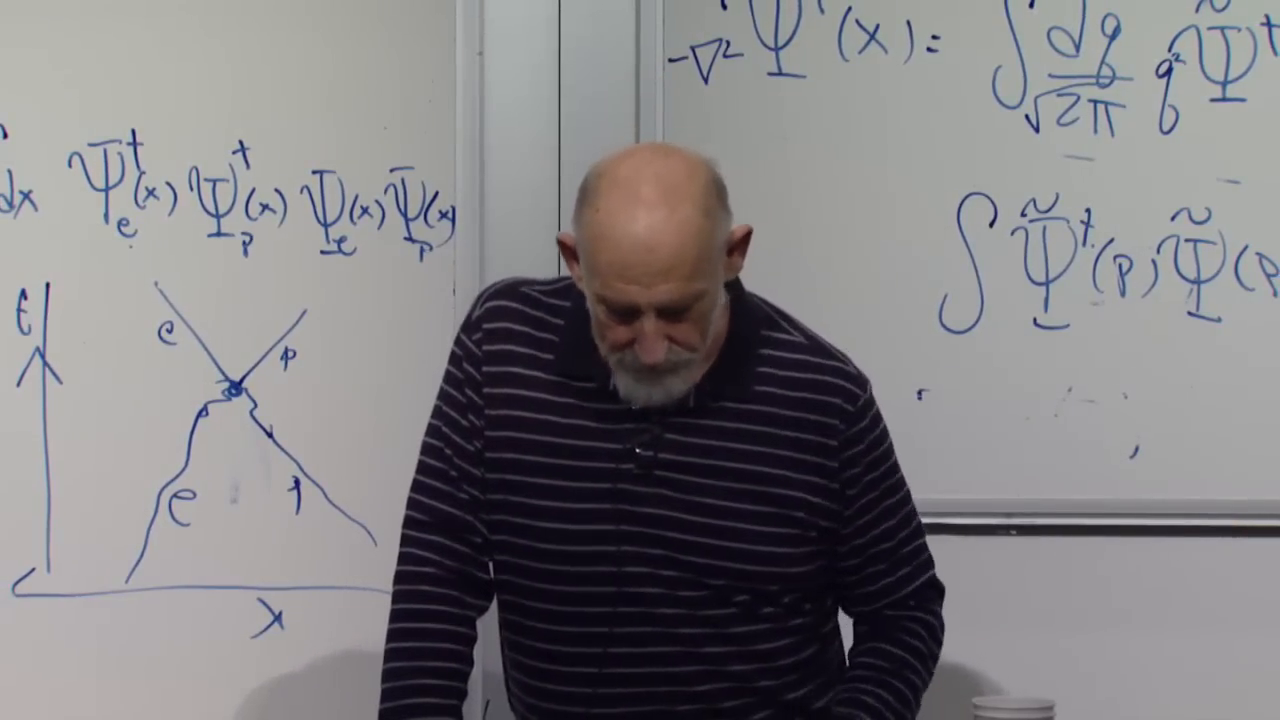
\includegraphics[width=0.94\linewidth]{lecture_09_frame_02.png}\caption{Tương tác tiếp xúc trên bảng. Bốn toán tử trường cục bộ được viết phía trên hình phác không thời gian; điểm gặp nhau là nơi duy nhất tương tác lý tưởng hóa này tác dụng.}\lectureframe{00:35:36}\end{figure}

\begin{figure}[htbp]\centering
\begin{tikzpicture}[x=1.2cm,y=1.0cm,>=Latex]
\draw[->] (-3.0,0) -- (3.0,0) node[right] {$x$};
\draw[->] (0,-0.2) -- (0,4.2) node[above] {$t$};
\coordinate (v) at (0,2.0);
\fill (v) circle (1.8pt);
\draw[thick,->] (-2.2,0.4) -- (v);
\draw[thick,->] (2.0,0.4) -- (v);
\draw[thick,->] (v) -- (-1.6,3.7);
\draw[thick,->] (v) -- (2.2,3.7);
\node[left] at (-1.65,0.7) {$e$};
\node[right] at (1.55,0.7) {$p$};
\node[left] at (-1.15,3.3) {$e$};
\node[right] at (1.65,3.3) {$p$};
\node[right] at (0.12,2.05) {$g$};
\end{tikzpicture}\caption{Bản dựng lại rõ ràng hình ảnh tán xạ cục bộ. Đỉnh là cách viết tắt cho toán tử trong Phương trình~\eqref{eq:l9-contact}, chứ không phải định luật va chạm cổ điển.}\end{figure}

Electron và proton thực tương tác từ xa thông qua thế Coulomb. Mô hình tiếp xúc chỉ là bước đầu ngắn gọn: nếu thực nghiệm cho thấy hai loài hạt chỉ tán xạ khi chúng chồng lấp, thì Phương trình~\eqref{eq:l9-contact} là dạng số hạng ta sẽ đưa vào Hamiltonian.

\begin{classroomqa}\lecturetimestamp{00:35:40}\audiencequestion{Vì sao toán tử tán xạ này lại nằm trong Hamiltonian nếu năng lượng không thay đổi?}\lecturerresponse{Hamiltonian vừa là toán tử năng lượng, vừa là toán tử sinh ra sự biến đổi của trạng thái. Thế năng giữa hai hạt gây ra tán xạ trong quá trình tiến hóa theo thời gian. Bảo toàn năng lượng toàn phần không có nghĩa là trạng thái, hay động lượng riêng lẻ của các hạt, không đổi.}\end{classroomqa}

Điều này cho ta một quy tắc thực hành. Trước hết, hãy tìm hiểu từ thực nghiệm những quá trình cục bộ mà các hạt có thể trải qua. Sau đó, mã hóa các quá trình ấy trong toán tử cập nhật trạng thái. Tích các trường không phải là phép biến đổi đại số để trang trí: các thừa số có dấu dagơ và không có dấu dagơ chỉ rõ loài hạt nào xuất hiện và biến mất.

\section{Phân rã, quá trình nghịch đảo và tính Hermite}

Giả sử buồng bọt cho thấy một vệt của loài \(A\) kết thúc tại một điểm, từ đó xuất hiện các vệt \(B\) và \(C\). Quá trình cục bộ là
\begin{equation}
A\longrightarrow B+C.
\end{equation}
Toán tử thực hiện quá trình đó là
\begin{equation}
V=g\int dx\,
\psi_B^\dagger(x)\psi_C^\dagger(x)\psi_A(x).
\label{eq:l9-decay-half}
\end{equation}
Trường hủy loại bỏ \(A\); hai trường tạo sinh ra \(B\) và \(C\) tại cùng một điểm. Tích phân với trọng số bằng nhau trên mọi \(x\) biểu thị tính bất biến tịnh tiến không gian và lập tức cho
\begin{equation}
p_A=p_B+p_C.
\end{equation}

Hamiltonian phải là toán tử Hermite. Điều này khiến \(e^{-itH}\) là toán tử đơn nhất và bảo toàn xác suất toàn phần. Phương trình~\eqref{eq:l9-decay-half} tự nó không phải Hermite, nên ta phải thêm toán tử liên hợp của nó:
\begin{equation}
H_{\mathrm{int}}
=\int dx\left[
g\,\psi_B^\dagger\psi_C^\dagger\psi_A
+g^*\,\psi_A^\dagger\psi_C\psi_B
\right](x).
\label{eq:l9-hermitian-vertex}
\end{equation}
Với hằng số tương tác thực \(g\), hai hệ số bằng nhau. Liên hợp Hermite đảo thứ tự toán tử, đồng thời hoán đổi các trường có dấu dagơ và không có dấu dagơ. Trong mô hình đồ chơi boson này, các trường thuộc những loài khác nhau giao hoán, nên việc đảo thứ tự không gây thêm phức tạp nào.

Số hạng thứ hai thực hiện quá trình nghịch đảo,
\begin{equation}
B+C\longrightarrow A.
\end{equation}
Vì thế, Hamiltonian kín và đơn nhất cho phép phân rã cũng chứa biên độ tái hợp. Điều đó không bảo đảm cả hai chiều đều xảy ra với mọi tập động lượng ngoài được chọn; các định luật bảo toàn năng lượng và những định luật khác có thể khiến một chiều không thể xảy ra về mặt động học. Điều đó có nghĩa là cả toán tử tương tác lẫn toán tử liên hợp của nó đều thuộc về động lực học.

\begin{classroomqa}\lecturetimestamp{00:42:48}\audiencequestion{Có ngoại lệ nào cho quy tắc rằng quá trình nghịch đảo cũng được phép xảy ra không?}\lecturerresponse{Không, nếu xét ở cấp Hamiltonian của một hệ kín Hermite: tương tác liên hợp là bắt buộc. Một phản ứng ngược cụ thể vẫn có thể bị cấm bởi động học hoặc một số lượng tử được bảo toàn khác, nhưng phần tử ma trận liên hợp vẫn hiện diện.}\end{classroomqa}

Số \(g\) là hằng số tương tác. Nếu \(g\) nhỏ, các hạt gặp nhau sẽ tương tác yếu; nếu nó lớn, biên độ chuyển tiếp lớn hơn. Các hằng số tương tác thường là những tham số được đo trong thực nghiệm, dù các đối xứng có thể liên hệ một số hằng số tưởng như khác nhau.

Cùng quy tắc biểu đạt này cũng mô tả được những phản ứng phức tạp hơn. Trong phân rã beta,
\begin{equation}
n\longrightarrow p+e^-+\bar\nu_e,
\end{equation}
một số hạng cục bộ sơ đồ chứa bốn trường: một trường hủy neutron, ba trường tạo proton, electron và phản neutrino electron, cùng với quá trình liên hợp Hermite. Chỉ vậy cũng đủ để thấy một tập nhỏ các đơn thức toán tử bắt đầu định hình một lý thuyết trường lượng tử như thế nào.

\section{Vì sao bình phương Hamiltonian lại quan trọng}

Công thức thời gian ngắn \eqref{eq:l9-short-update} chỉ giữ lại bậc nhất theo \(\epsilon\). Khai triển đầy đủ là
\begin{equation}
e^{-i\epsilon H}
=1-i\epsilon H-\frac{\epsilon^2}{2}H^2
+\frac{i\epsilon^3}{3!}H^3+\cdots.
\label{eq:l9-exponential}
\end{equation}
Ở bậc hai, Hamiltonian tác dụng hai lần. Đây là nguồn gốc đại số của những hình ảnh quá trình tổ hợp đầu tiên.

Với đỉnh \(A\leftrightarrow B+C\), một lần tác dụng có thể kết hợp \(B+C\) thành \(A\), còn lần thứ hai có thể phân rã \(A\) đó trở lại thành \(B+C\):
\begin{equation}
B+C\longrightarrow A\longrightarrow B+C.
\label{eq:l9-bc-scattering}
\end{equation}
Đóng góp thuần là một biên độ tán xạ \(B+C\to B+C\). Trạng thái trung gian \(A\) không phải là một sự kiện quan sát được bổ sung; nó chỉ trạng thái được lấy tổng qua giữa hai lần tương tác tác dụng.

\begin{classroomqa}\lecturetimestamp{00:49:54}\audiencequestion{Trường \(C\) trong tích toán tử bậc hai được viết trên bảng có cần mang dấu dagơ không?}\lecturerresponse{Có, thứ tự toán tử phải khớp với trình tự đã nêu. Đỉnh thứ nhất hủy \(B\) và \(C\), đồng thời tạo \(A\); đỉnh thứ hai hủy \(A\) rồi tạo lại \(B\) và \(C\). Viết đúng các dấu dagơ tương ứng sẽ khôi phục cách diễn giải ấy.}\end{classroomqa}

\begin{figure}[htbp]\centering
\includegraphics[width=0.94\linewidth]{lecture_09_frame_05.png}\caption{Hai chiều của đỉnh cơ bản \(A\leftrightarrow B+C\) trên bảng. Đặt chúng cạnh nhau là cách biểu diễn trực quan tắt gọn cho quá trình bậc hai trong Phương trình~\eqref{eq:l9-bc-scattering}.}\lectureframe{00:48:56}\end{figure}

Giờ thêm một hạt \(B\) làm nhân chứng. Một lần tương tác cho phép \(A\) phát ra \(C\) và biến thành \(B\); lần tương tác sau cho phép \(C\) ấy kết hợp với \(B\) ban đầu để tạo thành \(A\). Các hạt ngoài vẫn là \(A+B\), nhưng động lượng của chúng có thể thay đổi. Ta mô tả đây là tán xạ \(A\) và \(B\) thông qua trao đổi \(C\).

\begin{figure}[htbp]\centering
\includegraphics[width=0.94\linewidth]{lecture_09_frame_06.png}\caption{Cách dựng quá trình trao đổi trên bảng. Giản đồ bên phải nối hai đỉnh cơ bản bằng một đường \(C\) nội tại, trong khi các hạt \(A\) và \(B\) bên ngoài tán xạ.}\lectureframe{00:51:22}\end{figure}

\begin{figure}[htbp]\centering
\begin{tikzpicture}[x=1.1cm,y=1cm,>=Latex]
\draw[->] (-3.7,-0.2) -- (-3.7,4.2) node[above] {$t$};
\coordinate (v1) at (-0.9,1.25);
\coordinate (v2) at (0.9,2.95);
\fill (v1) circle (1.7pt);
\fill (v2) circle (1.7pt);
\draw[thick,->] (-2.6,0.2) -- (v1) node[midway,below left] {$A$};
\draw[thick,->] (2.6,0.2) -- (v2) node[midway,below right] {$B$};
\draw[thick,->] (v1) -- (-2.4,4.0) node[midway,left] {$B$};
\draw[thick,->] (v2) -- (2.5,4.0) node[midway,right] {$A$};
\draw[thick,->,dashed] (v1) -- (v2) node[midway,above left] {$C$};
\node[below] at (0,-0.05) {$A+B\rightarrow A+B$};
\end{tikzpicture}\caption{Bản dựng lại rõ ràng quá trình trao đổi \(C\). Mỗi chấm đóng góp một thừa số \(g\), nên số hạng bậc hai này tỷ lệ với \(g^2\).}\end{figure}

Mỗi điểm tương tác cục bộ được gọi là một đỉnh. Mỗi đỉnh đóng góp một thừa số bằng hằng số tương tác của nó, vì thế đóng góp có hai đỉnh chứa \(g^2\), đóng góp có ba đỉnh chứa \(g^3\), vân vân. Do đó, một số hạng duy nhất trong Hamiltonian tương quan hóa được cả một họ phản ứng lớn. Đây là một lý do khiến lý thuyết trường lượng tử mạnh mẽ đến vậy: một số ít tương tác cục bộ có thể sắp xếp một lượng dữ liệu tán xạ khổng lồ.

\begin{classroomqa}\lecturetimestamp{00:53:14}\audiencequestion{Quá trình \(A\to B+C\to A\) được gọi là gì?}\lecturerresponse{Đó là một đóng góp tự năng. Một \(A\) được đo không chỉ là trạng thái cơ sở một hạt trần; trạng thái tương tác còn có biên độ cho các thành phần \(B+C\) lân cận. Tán xạ với trạng thái ấy có thể cho thấy cấu trúc đã được bao quanh đó.}\end{classroomqa}

Điện động lực học lượng tử đưa ra ví dụ quen thuộc. Một đỉnh electron--photon cục bộ có thể hủy một electron, tạo lại một electron và tạo ra một photon. Ở bậc hai, electron có thể phát ra rồi tái hấp thụ một photon. Ta dễ bị cám dỗ kể lại điều này như một đoạn phim tí hon, nhưng ý nghĩa chặt chẽ của nó chỉ là một số hạng trong khai triển nhiễu loạn. Electron vật lý là một trạng thái đã được bao quanh, có các thành phần chứa photon.

Ước lượng trong lớp học rằng thành phần này là ``khoảng một phần trăm'' cho thấy quy mô do hằng số cấu trúc tinh tế quyết định, \(\alpha_{\mathrm{em}}\simeq 1/137\). Xác suất chính xác cho một thành phần Fock chứa photon phụ thuộc vào độ phân giải năng lượng và cách định nghĩa trạng thái tương tác; đó không phải là thuộc tính một phần trăm phổ quát của một electron cô lập. Phát biểu vững chắc là tương tác làm thay đổi cấu trúc đo được của electron.

\section{Giản đồ cho biết điều gì và không cho biết điều gì}

Các giản đồ là cách viết tắt phục vụ tính toán cho các lũy thừa của Hamiltonian tương tác. Chúng không phải những diễn biến cổ điển đáng tin cậy, trong đó một hạt chắc chắn thực hiện sự kiện này rồi đến sự kiện khác. Việc nhìn vào bên trong để quyết định phương án trung gian nào đã ``thực sự xảy ra'' sẽ làm thay đổi thí nghiệm và phá hủy tổng kết hợp, cũng như trong giao thoa lượng tử thông thường.

\begin{classroomqa}\lecturetimestamp{00:56:52}\audiencequestion{Tại đỉnh đầu tiên, cả năng lượng lẫn động lượng có được bảo toàn không?}\lecturerresponse{Trong cách xây dựng Hamiltonian tại thời điểm bằng nhau được thực hiện ở đây, tích phân không gian lập tức tạo ra một hàm delta động lượng. Tích phân theo thời gian chưa tạo ra hàm delta năng lượng cho phép chèn riêng lẻ đó. Biên độ tán xạ đầy đủ bất biến tịnh tiến theo thời gian bảo toàn năng lượng toàn phần, còn các đường nội tại không nhất thiết tuân theo hệ thức trên vỏ của các hạt quan sát được. Trong ngôn ngữ giản đồ hiệp biến, bốn động lượng được bảo toàn tại mỗi đỉnh, nhưng các hạt nội tại có thể nằm ngoài vỏ.}\end{classroomqa}

Năng lượng dường như bị thiếu trong hình dung ngây thơ về một đỉnh là lời nhắc khác rằng không được bỏ qua năng lượng tương tác. Hamiltonian toàn phần không chỉ là tổng năng lượng của các hạt tự do. Nếu thấy khó hiểu, hãy quay lại Phương trình~\eqref{eq:l9-exponential}: hình vẽ biểu diễn một số hạng trong khai triển tiến hóa đơn nhất theo thời gian. Công cụ giản đồ Feynman đầy đủ cung cấp cách sắp thứ tự thời gian, các hàm truyền, phép tích phân và các hệ số đối xứng một cách có hệ thống, nhưng vật lý cơ bản bắt đầu từ đây.

Một câu hỏi mở rộng diễn giải giản đồ quá sát nghĩa khi so sánh photon phát ra với điện trường bao quanh một electron chuyển động chậm.

\begin{classroomqa}\lecturetimestamp{00:58:26}\audiencequestion{Điện trường của electron ở khoảng cách xa có thực sự do các photon bức xạ tạo ra không? Điều đó liên hệ thế nào với giao thoa và hiệu ứng Aharon--Bohm?}\lecturerresponse{Trường tĩnh hoặc trường cảm ứng không phải là dòng photon bức xạ thực. Điện động lực học lượng tử mô tả cả bức xạ lẫn sự bao quanh điện từ của electron bằng cùng một trường, nhưng các trạng thái lượng tử và động học tương ứng khác nhau. Với electron siêu tương đối tính, một số thành phần trường có thể được xem hữu ích như một dòng photon gần thực; với electron chậm, hình dung quỹ đạo photon theo nghĩa đen là không phù hợp. Giao thoa hai khe và hiệu ứng Aharon--Bohm cũng là những hiện tượng trường phi cổ điển, nhưng chúng không biến giản đồ tự năng này thành một đoạn phim cơ học.}\end{classroomqa}

\begin{classroomqa}\lecturetimestamp{01:01:28}\audiencequestion{Chính xác thì vì sao mô hình cổ điển của giản đồ lại thất bại?}\lecturerresponse{Vì phép tính cộng kết hợp các biên độ của mọi phương án trung gian được phép. Kinh nghiệm khiến các hình vẽ trở nên trực quan, nhưng ý nghĩa theo nghĩa đen của chúng không bao giờ vượt quá khai triển toán tử định nghĩa chúng. Chúng là cách tính gọn cho \(H^2,H^3,\ldots\), chứ không phải bản ghi những sự kiện trung gian đã được quan sát.}\end{classroomqa}

\begin{classroomqa}\lecturetimestamp{01:03:04}\audiencequestion{Tương tác Coulomb thông thường có thể xuất hiện như giới hạn cổ điển của quá trình trao đổi photon không?}\lecturerresponse{Có. Tính biên độ thích hợp do photon trung gian và lấy giới hạn tĩnh phi tương đối tính sẽ cho thế Coulomb. Phép suy dẫn này phức tạp hơn phần phác họa toán tử ở đây, và cũng không nên được hiểu là photon thực sự nhảy giữa hai hạt cổ điển.}\end{classroomqa}

\begin{classroomqa}\lecturetimestamp{01:03:44}\audiencequestion{Các hằng số tương tác có được tính từ tích các trường không?}\lecturerresponse{Thông thường, giá trị số của chúng là dữ liệu đầu vào từ thực nghiệm. Đối xứng có thể ràng buộc chúng hoặc liên hệ các hằng số vốn dĩ sẽ độc lập. Khi một quan hệ như vậy dự đoán độ mạnh tương đối của những phản ứng khác nhau và thực nghiệm xác nhận điều đó, sự phù hợp đặc biệt có ý nghĩa.}\end{classroomqa}

\begin{classroomqa}\lecturetimestamp{01:04:48}\audiencequestion{Đối xứng ngẫu nhiên khác đối xứng chuẩn tắc như thế nào về vai trò?}\lecturerresponse{Đối xứng chuẩn tắc trực tiếp ràng buộc cấu trúc được phép và các quan hệ giữa những hằng số tương tác. Đối xứng ngẫu nhiên không được áp đặt ở cấp cơ bản, mà xuất hiện vì mọi tương tác được phép ở bậc thấp hơn tình cờ đều tôn trọng nó. Đối xứng ấy vẫn có thể dẫn đến những hệ quả quan trọng, dù nguồn gốc và độ bền vững khác với đối xứng chuẩn tắc.}\end{classroomqa}

Tạm thời, thế là đủ về lý thuyết trường phi tương đối tính. Ta đã hứa sẽ nói về fermion. Thay vì lượng tử hóa lần hai chúng ngay lập tức, trước hết ta sẽ tìm hiểu phương trình một hạt tương đối tính mà các toán tử trường của chúng phải thỏa mãn.

\section{Vì sao electron cần đến thuyết tương đối}

Bắt đầu với một chiều không gian. Đây không phải là hạn chế thực tế, nhưng nó loại bỏ sự phức tạp hình học của spin trong ba chiều mà vẫn giữ nguyên phần đại số cốt yếu. Electron đủ nhẹ để hiệu ứng tương đối tính quan trọng ngay cả trong nguyên tử. Trong nguyên tử hydro, tốc độ đặc trưng của nó cỡ
\begin{equation}
v\sim\alpha_{\mathrm{em}}c\approx 0.007c,
\end{equation}
xấp xỉ một phần trăm tốc độ ánh sáng. Với các electron lớp trong của nguyên tử nặng, thang ước lượng trở thành \(v\sim Z\alpha_{\mathrm{em}}c\), nên hiệu chỉnh tương đối tính có thể đáng kể. Dù động lực quyết định là sự tò mò lịch sử hay độ chính xác trong vật lý nguyên tử, một phương trình kiểu Schr\"odinger tương đối tính vẫn cần thiết về mặt vật lý.

Cách lượng tử hóa thông thường bắt đầu từ hệ thức cổ điển giữa năng lượng và động lượng. Trong giới hạn phi tương đối tính,
\begin{equation}
E=\frac{p^2}{2m},
\end{equation}
và các phép thay thế
\begin{equation}
E\mapsto i\partial_t,
\qquad
p\mapsto-i\partial_x
\end{equation}
cho
\begin{equation}
i\partial_t\varphi(x,t)
=-\frac{1}{2m}\partial_x^2\varphi(x,t).
\end{equation}

Thuyết tương đối thay vào đó cho hệ thức, với \(c=1\),
\begin{equation}
E^2=p^2+m^2.
\label{eq:l9-rel-dispersion}
\end{equation}

\begin{figure}[htbp]\centering
\includegraphics[width=0.94\linewidth]{lecture_09_frame_07.png}\caption{Bước chuyển trên bảng từ \(E=p^2/2m\) sang hệ thức tương đối tính \(E^2=p^2+m^2\), với \(c=1\).}\lectureframe{01:10:30}\end{figure}

Áp dụng các phép thay thế vào hệ thức bình phương cho
\begin{equation}
-\partial_t^2\varphi
=\left(-\partial_x^2+m^2\right)\varphi,
\label{eq:l9-klein-gordon}
\end{equation}
hoặc tương đương
\begin{equation}
\left(\partial_t^2-\partial_x^2+m^2\right)\varphi=0.
\end{equation}
Đây là phương trình Klein--Gordon. Đây là một phương trình trường tương đối tính hoàn toàn có ý nghĩa, đặc biệt đối với các trường spin không. Nhưng phương trình electron ta cần phải bậc nhất theo thời gian,
\begin{equation}
i\partial_t\Psi=H\Psi,
\end{equation}
để chính \(H\), chứ không chỉ \(H^2\), sinh ra sự tiến hóa.

Về hình thức, ta có thể chọn
\begin{equation}
H=\sqrt{-\partial_x^2+m^2}.
\end{equation}
Căn bậc hai có thể được định nghĩa rõ ràng trong không gian động lượng, nơi nó nhân với \(\sqrt{p^2+m^2}\), nhưng trong không gian vị trí, nó là một toán tử giả vi phân phi cục bộ. Toán tử này có ý nghĩa kỹ thuật, nhưng không hữu ích về mặt thẩm mỹ cho phương trình cục bộ mà ta đang tìm. Vì vậy, ta bắt đầu lại.

\section{Sóng không khối lượng chuyển động sang phải}

Trước hết, xét một hạt không khối lượng chuyển động sang phải. Năng lượng dương và động lượng của nó thỏa mãn
\begin{equation}
E=p
\qquad (c=1).
\end{equation}
Lượng tử hóa cho
\begin{equation}
i\partial_t\psi=-i\partial_x\psi,
\end{equation}
hoặc
\begin{equation}
(\partial_t+\partial_x)\psi=0.
\label{eq:l9-right-mover}
\end{equation}
Mọi nghiệm đều có dạng
\begin{equation}
\psi(x,t)=f(x-t).
\end{equation}
Dạng sóng giữ nguyên hình dạng và chuyển động sang phải với tốc độ ánh sáng.

Hai khó khăn xuất hiện ngay lập tức. Thứ nhất, nếu cho phép Phương trình~\eqref{eq:l9-right-mover} tác dụng lên các mode Fourier tùy ý, động lượng âm có năng lượng \(E=p<0\), nên Hamiltonian không bị chặn dưới. Nếu tự áp đặt điều kiện \(p>0\), ta chỉ giữ lại các sóng chuyển động sang phải, và đó vẫn chưa phải lý thuyết electron mà ta cần. Thứ hai, phương trình này chỉ cho phép chuyển động theo một chiều: nó không chứa electron thông thường chuyển động sang trái. Trước hết, ta sẽ giải quyết vấn đề trái-phải, còn để nguyên các năng lượng âm.

\section{Hai thành phần và ma trận alpha}

Đưa vào hai biên độ,
\begin{equation}
\Psi(x,t)=
\begin{pmatrix}
\psi_1(x,t)\\[3pt]
\psi_2(x,t)
\end{pmatrix},
\end{equation}
trong đó \(\psi_1\) chuyển động sang phải và \(\psi_2\) chuyển động sang trái trong giới hạn không khối lượng:
\begin{align}
(\partial_t+\partial_x)\psi_1&=0,
&
(\partial_t-\partial_x)\psi_2&=0.
\end{align}
Cơ học lượng tử cũng cho phép chồng chập tùy ý của hai thành phần này. Vì vậy, một hạt có thể có biên độ ứng với cả hai hướng, thay vì mang một nhãn cổ điển được chọn một lần rồi giữ nguyên.

Bậc tự do hai trị bổ sung này giống spin về mặt đại số, nhưng trong một chiều nó không phải là mômen động lượng thông thường. Định nghĩa
\begin{equation}
\alpha=
\begin{pmatrix}
1&0\\
0&-1
\end{pmatrix}
=\sigma_3.
\label{eq:l9-alpha}
\end{equation}
Các vectơ riêng ứng với trị riêng \(+1\) của nó chọn thành phần truyền sang phải, còn các vectơ riêng ứng với trị riêng \(-1\) chọn thành phần truyền sang trái. Trong lý thuyết không khối lượng, Hamiltonian có dạng đơn giản
\begin{equation}
H=\alpha p,
\end{equation}
và hai phương trình hợp thành
\begin{equation}
i\partial_t\Psi=-i\alpha\partial_x\Psi.
\label{eq:l9-massless-dirac}
\end{equation}

\begin{classroomqa}
\lecturetimestamp{01:22:44}
\audiencequestion{Ma trận đường chéo phân biệt hai thành phần có tên gọi là gì?}
\lecturerresponse{Nếu xét như một ma trận Pauli, đó là \(\sigma_3\), chứ không phải \(\sigma_1\). Trong ký hiệu Dirac dùng cho cấu trúc đang xét, ta gọi nó là \(\alpha\). Đại số của nó chính là đại số Pauli quen thuộc, dù ở đây nhãn vật lý là chiều truyền chứ không phải mômen động lượng spin.}
\end{classroomqa}

\begin{classroomqa}
\lecturetimestamp{01:23:32}
\audiencequestion{Trong ba chiều, khi hướng là một vectơ, cấu trúc này có ý nghĩa hình học rõ hơn không?}
\lecturerresponse{Có. Bài toán ba chiều cần một ma trận cho mỗi phương không gian và dẫn đến cấu trúc spinor phong phú hơn. Dù vậy, mô hình một chiều vẫn chính xác trong phạm vi của nó và tách riêng đại số trái-phải cốt yếu mà không có phần phức tạp bổ sung đó.}
\end{classroomqa}

\begin{figure}[htbp]
\centering
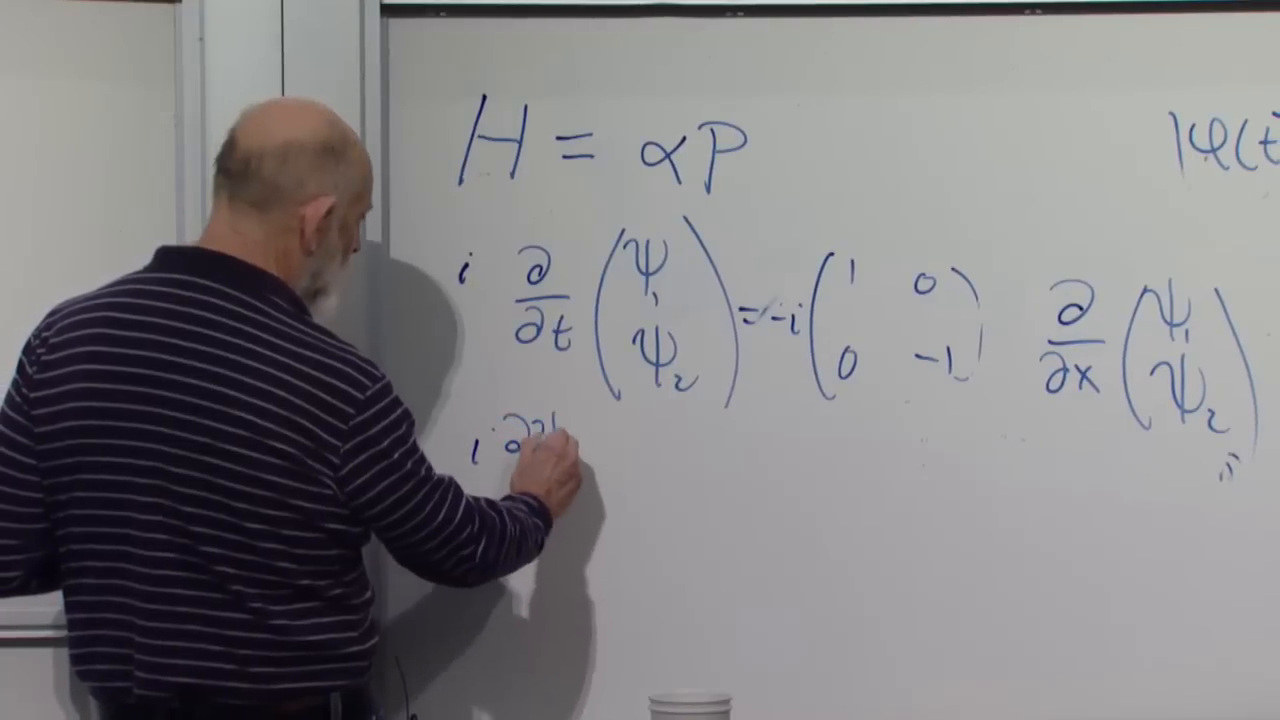
\includegraphics[width=0.94\linewidth]{lecture_09_frame_03.png}
\caption{Phương trình hai thành phần không khối lượng trên bảng: \(H=\alpha P\), trong đó ma trận đường chéo gán chiều truyền ngược nhau cho \(\psi_1\) và \(\psi_2\).}
\lectureframe{01:26:00}
\end{figure}

Bài toán chỉ có một chiều truyền đã được giải quyết. Phổ năng lượng âm vẫn còn đó, và ta phát hiện ra khiếm khuyết thứ ba: hai thành phần vẫn không có khối lượng và truyền đi với tốc độ ánh sáng. Bước tiếp theo phải đưa năng lượng nghỉ vào và ghép hai chiều truyền với nhau.

\section{Thêm khối lượng và khám phá đại số Dirac}

Thêm số hạng đơn giản tổng quát nhất tỉ lệ với khối lượng,
\begin{equation}
H=\alpha p+\beta m,
\label{eq:l9-dirac-hamiltonian}
\end{equation}
trong đó \(\beta\) chỉ tác động lên chỉ số hai thành phần. Số hạng này có thể là ma trận đơn vị hoặc một ma trận khác; ta để hệ thức tán sắc tương đối tính quyết định.

Vì \(H^2\) phải bằng \(p^2+m^2\), hãy bình phương phương trình ~\eqref{eq:l9-dirac-hamiltonian}:
\begin{align}
H^2
&=(\alpha p+\beta m)^2\\
&=\alpha^2p^2+\beta^2m^2
+(\alpha\beta+\beta\alpha)pm.
\label{eq:l9-square-dirac}
\end{align}
Các ma trận giao hoán với \(p\) vì chúng tác động lên không gian nội tại hai thành phần, còn \(p\) tác động lên hàm sóng không gian. Để khớp với phương trình ~\eqref{eq:l9-rel-dispersion}, cần có
\begin{equation}
\alpha^2=\mathbb{1},
\qquad
\beta^2=\mathbb{1},
\qquad
\{\alpha,\beta\}
=\alpha\beta+\beta\alpha=0.
\label{eq:l9-dirac-algebra}
\end{equation}
Điều kiện thứ nhất đã được thỏa mãn với \(\alpha=\sigma_3\). Mọi ma trận Pauli khác đều phản giao hoán với nó và bình phương thành ma trận đơn vị. Chọn
\begin{equation}
\beta=
\begin{pmatrix}
0&1\\
1&0
\end{pmatrix}
=\sigma_1.
\label{eq:l9-beta}
\end{equation}
Việc chọn \(\sigma_1\) thay vì \(\sigma_2\) chỉ là quy ước cơ sở; cả hai đều hiện thực hóa cùng một đại số sau một phép đổi cơ sở unita.

\begin{classroomqa}
\lecturetimestamp{01:33:00}
\audiencequestion{Dirac có đơn giản là nhận ra các ma trận Pauli thỏa mãn những điều kiện đại số này không?}
\lecturerresponse{Phép suy dẫn trong lịch sử được thực hiện trực tiếp trong ba chiều và đưa vào các ma trận thỏa mãn những hệ thức cần thiết. Khi đã viết ra các điều kiện, đại số Pauli cho thấy ngay nghiệm một chiều: chọn hai ma trận Pauli khác nhau.}
\end{classroomqa}

\begin{classroomqa}
\lecturetimestamp{01:34:24}
\audiencequestion{Đây có phải là tham số vận tốc tương đối tính \(\beta\) không?\(v/c\)}
\lecturerresponse{Không. Đây là một ma trận tác động lên các thành phần spinor. Chữ cái được dùng lại chỉ là ký hiệu của Dirac; nó không liên quan gì đến đại lượng động học \(v/c\).}
\end{classroomqa}

Trong ba chiều không gian, các ma trận \(2\times2\) là không đủ để tạo thành tập đầy đủ các ma trận phản giao hoán cần thiết. Ta sẽ xét việc mở rộng đó sau. Trong một chiều, các phương trình ~\eqref{eq:l9-alpha} và \eqref{eq:l9-beta} là đủ.

\section{Phương trình Dirac một chiều có ghép nối}

Thay \(p=-i\partial_x\) vào, ta thu được phương trình Dirac một chiều ở dạng Hamiltonian:
\begin{equation}
i\partial_t\Psi
=\left(-i\alpha\partial_x+\beta m\right)\Psi.
\label{eq:l9-one-dimensional-dirac}
\end{equation}
Vì \(\alpha\) là ma trận đường chéo nên số hạng đạo hàm giữ hai thành phần tách biệt. Vì \(\beta\) là ma trận ngoài đường chéo nên số hạng khối lượng hoán đổi chúng cho nhau. Viết riêng từng thành phần,
\begin{align}
i\partial_t\psi_1
&=-i\partial_x\psi_1+m\psi_2,
\label{eq:l9-dirac-component-one}\\
i\partial_t\psi_2
&=+i\partial_x\psi_2+m\psi_1.
\label{eq:l9-dirac-component-two}
\end{align}

\begin{figure}[htbp]
\centering
\includegraphics[width=0.94\linewidth]{lecture_09_frame_08.png}
\caption{Các phương trình thành phần có ghép nối trên bảng. Dấu đạo hàm trái ngược nhau biểu thị chuyển động sang phải và sang trái; số hạng khối lượng ngoài đường chéo hoán đổi \(\psi_1\) và \(\psi_2\).}
\lectureframe{01:37:44}
\end{figure}

Các thành phần không còn tiến hóa độc lập ngay khi \(m\ne0\). Bình phương phương trình bậc nhất thu lại toán tử Klein--Gordon trên mỗi thành phần,
\begin{equation}
\left(\partial_t^2-\partial_x^2+m^2\right)\psi_a=0,
\qquad a=1,2,
\end{equation}
và sóng phẳng thỏa mãn \(E^2=p^2+m^2\). Vận tốc nhóm của chúng là
\begin{equation}
v_g=\frac{dE}{dp}=\frac{p}{E},
\end{equation}
độ lớn của vận tốc này nhỏ hơn một khi khối lượng khác không.

Mối liên hệ giữa khối lượng và sự trộn lẫn trái-phải không phải là ngẫu nhiên. Một hạt chuyển động sang phải không khối lượng vẫn chuyển động sang phải dưới mọi phép biến đổi Lorentz chính tắc; không người quan sát nào chuyển động dưới ánh sáng có thể vượt qua ánh sáng rồi đảo chiều truyền của nó. Một hạt có khối lượng có thể được đưa về trạng thái nghỉ, rồi được quan sát từ một hệ quy chiếu chuyển động nhanh hơn theo cùng chiều, trong đó vận tốc của nó có vẻ như đã đảo chiều. Vì vậy, lý thuyết tương đối tính có khối lượng không thể giữ các khu vực trái và phải tách biệt vĩnh viễn. Số hạng khối lượng ngoài đường chéo tạo ra chính xác sự ghép nối cần thiết.

\begin{classroomqa}
\lecturetimestamp{01:40:01}
\audiencequestion{Sự hoán đổi hai thành phần có phải là dao động chiral không?}
\lecturerresponse{Trong cơ sở một chiều này, \(\alpha\) phân biệt hai chiều chiral không khối lượng. Số hạng khối lượng nằm ngoài đường chéo và trộn lẫn chúng, vì thế tính chiral không còn được bảo toàn. Theo nghĩa đó, số hạng khối lượng là nguồn gốc của dao động chiral.}
\end{classroomqa}

\begin{classroomqa}
\lecturetimestamp{01:40:46}
\audiencequestion{Vì sao phương trình của fermion lại phải là căn bậc hai của phương trình boson?}
\lecturerresponse{Không nên hiểu vấn đề theo cách đó. Hệ thức tán sắc \(E^2=p^2+m^2\) áp dụng cho mọi hạt tương đối tính tự do, bất kể thống kê. Toán tử Dirac tình cờ cho ta một phép phân tích nhân tử dạng ma trận của toán tử Klein--Gordon, nhưng quan hệ đại số đó không suy ra fermion từ boson.}
\end{classroomqa}

\begin{classroomqa}
\lecturetimestamp{01:41:31}
\audiencequestion{Có thể phân tích phương trình thành các nhân tử vô hướng đơn giản, tách riêng phần truyền sang trái và sang phải không?}
\lecturerresponse{Chỉ trong giới hạn không khối lượng thì hai phương trình chiral mới tách thành các nhân tử vô hướng độc lập. Khi \(m\ne0\), phép phân tích nhân tử hữu ích có dạng ma trận: chính các ma trận phản giao hoán \(\alpha\) và \(\beta\) loại bỏ số hạng chéo không mong muốn.}
\end{classroomqa}

\begin{classroomqa}
\lecturetimestamp{01:42:04}
\audiencequestion{Hai phương trình có ghép nối này đã cấu thành phương trình Dirac chưa?}
\lecturerresponse{Đúng. Kết hợp lại, chúng là phương trình Dirac trong một chiều không gian, tương đương với dạng gọn ở phương trình ~\eqref{eq:l9-one-dimensional-dirac}. Có thể thu được một ký hiệu hiệp biến đối xứng hơn bằng cách nhân với \(\beta\), nhưng ta sẽ để dạng đó lại phần sau.}
\end{classroomqa}

Cố ý còn để dở hai việc. Cấu trúc này chưa loại bỏ năng lượng âm; nó cung cấp nghiệm năng lượng âm trong cả hai khu vực có hướng truyền, khiến vấn đề ấy trở nên rõ ràng hơn chứ không bớt đi. Và lý thuyết vẫn chỉ tồn tại trong một chiều không gian. Diễn giải các nghiệm năng lượng âm và mở rộng đại số ma trận lên \(3+1\) chiều là những bước tiếp theo.
